\documentclass[dvipsnames,tikz]{standalone}
\usepackage{amsmath}
\usepackage{arevmath}
\usepackage{xcolor}
\usepackage{tikz}
\usetikzlibrary{calc}
\usetikzlibrary{decorations.pathreplacing,calligraphy,3d}

\tikzset{main/.style={draw=black, circle, color=black}}


\begin{document}
	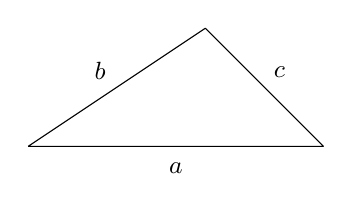
\begin{tikzpicture}[scale=0.75, main, line join=bevel]
		\draw[main] (0,0) -- (5,0) -- (3,2) -- cycle;
		\draw[font=\small, main] (2.5,0) node [below] {$a$};
		\draw[font=\small, main] (1.5,1) node [above left] {$b$};
		\draw[font=\small, main] (3+1,1) node [above right] {$c$};
	\end{tikzpicture}
\end{document}